\documentclass{hwset}

% info for header block in upper right hand corner
\name{Erich L Foster}
\class{Calculus I}
\duedate{Due: 31 January 2011}
\assignment{Homework 2}

\begin{document}
\begin{problem}[1.]
	\be 
		\item Evaluate $\lim_{x\to 2}\dfrac{x-2}{\sqrt{3-x}-1}$.
		\item Is there any number $a$ such that
		\begin{equation*}
			\lim_{x\to-2}\dfrac{3x^{2}+ax+a+3}{x^2+x-2}
		\end{equation*}
		exists? If so, find the value $a$ and the value of the limit.
	\ee
\end{problem}

\be
\item
\begin{solution}
	\begin{align*}
		\lim_{x\to 2} \dfrac{x-2}{\sqrt{3-x}-1} &= \lim_{x\to 2}
			\dfrac{x-2}{\sqrt{3-x}-1} \cdot \dfrac{\sqrt{3-x}+1}{\sqrt{3-x}+1} \\
		&= \lim_{x\to 2} \dfrac{(x-2)\left(\sqrt{3-x}+1\right)}{3-x-1} \\
		&= \lim_{x\to 2} \dfrac{(x-2)\left(\sqrt{3-x}+1\right)}{-(x-2)} \\
		&= -\lim_{x\to 2} \sqrt{3-x}+1 \\
		&= -\sqrt{3-2}+1 \\
		&= \boxed{-2.} 
	\end{align*}
\end{solution}
\item
\begin{solution}
	For this limit to exist we must require the limit be finite, i.e.
	\begin{equation*}
		\lim_{x\to-2}\dfrac{3x^{2}+ax+a+3}{x^2+x-2} < \infty
	\end{equation*}
	The easiest way to insure this is to make sure the factor $x+2$ in the
	denominator is canceled by a similar factor in the numerator. If we let the
	second factor in the numerator be $x+b$ then
	\begin{align*}
			3\left(x^{2}+\frac{a}{3}x+\frac{a}{3}+1\right) &= 3(x+2)(x+b) \\ 
			&= 3(x^2 + (2+b)x + 2b) 
	\end{align*}
	and therefore we must have
	\begin{align*}
		(2+b) &= \frac{a}{3} \\
		2b &= \frac{a}{3} + 1.
	\end{align*}
	Fom here we can solve for $b$ and $a$
	\begin{align*}
		b &= \frac{a + 3}{6} \\
		\Rightarrow 2 + \frac{a + 3}{6} &= \frac{a}{3} \\
		\frac{a + 3}{6} - \frac{a}{3} &= -2 \\
		a + 3 - 2a &= -12 \\
		a &= \boxed{15.} \Rightarrow b = 3 
	\end{align*}
	Now we just find the limit
	\begin{align*}
		\lim_{x\to -2} \dfrac{3(x+2)(x+3)}{(x+2)(x-1)} &= \lim_{x\to -2} \dfrac{3(x+3)}{x-1} \\
		&= \frac{3(-2+3)}{-2-1} \\
		&= \boxed{1.}
	\end{align*}
\end{solution}
\ee

\begin{problem}[2.]\S 2.3: 42.
\end{problem}

\begin{solution}
	\begin{align*}
		f(x) &= \begin{cases} x^2, & x\ne 1 \\ 2, & x=1 \end{cases} \\
		L &= 2 \\
		x_0 &= -2
	\end{align*}
	Substituting these into the limit definition and reducing to $a < x <b$
	\begin{align*}
		\left|x^2 - 4\right| &< \epsilon \\
		-\epsilon < x^2 - 4 &< \epsilon \\
		4 - \epsilon < x^2 &< \epsilon + 4 \\
		\text{Assuming }& \epsilon < 4 \text{ and using the negative square root}\\
		-\sqrt{4 - \epsilon} > x &> -\sqrt{\epsilon + 4}
	\end{align*}
	Additionally,
	\begin{align*}
		|x+2| &< \delta \\
		-\delta < x + 2 &< \delta \\
		-2 - \delta < x &< -2 + \delta \\
	\end{align*}
	From this we see that 
	\begin{align*}
		-2 - \delta &= -\sqrt{4 + \epsilon} \\
		\Rightarrow \delta &= \sqrt{4 + \epsilon} - 2 \\
		-2 + \delta &= 2 - \sqrt{4 - \epsilon} \\
		\Rightarrow \delta &= 2 - \sqrt{4 - \epsilon} \\
		\delta &= \min(\sqrt{4 + \epsilon} - 2, 2 - \sqrt{4 - \epsilon}) 
	\end{align*}
	Therefore, given $\epsilon > 0$ there exists a $\delta$ such that 
	\begin{equation*}
		0<|x + 2|<\epsilon \Rightarrow |f(x) - 4| < \epsilon.
	\end{equation*}
	\tbf{NOTE:} If $\epsilon > 4$ then we would take $\delta$ to be the distance
	from $x_0$ to the nearer endpoint of the interval $(-\sqrt{4 + \epsilon},0)$.
	Therefore,
	\begin{align*}
		-2 - \delta &= -\sqrt{4 + \epsilon} \\
		\Rightarrow \delta &= \sqrt{4 + \epsilon} - 2 \\
		-2 + \delta &= 0 \\
		\Rightarrow \delta &= 2 \\
		\delta = \min(2, \sqrt{4 + \epsilon} - 2)
	\end{align*}
\end{solution}

\begin{problem}[3.]\S 2.3: 55.
\end{problem}

\begin{solution}
	\begin{align*}
		f(x) &= \frac{\pi}{4} x^2 \\
		L &= 9 \text{in}^2 \\
		x_0 &= 3.385 \text{in} \\
		\epsilon &= 0.01 \text{in}^2
	\end{align*}
	We are looking for a $\delta$ defined in the same way that we used in the limit
	definition, and so we will reduce $|f(x) - L| < \epsilon$ to $a < x < b$, so
	that we can determine the tolerance $\delta$.
	\begin{align*}
		\left|\frac{\pi}{4} x^2 - 9\right| &< 0.01 \\
		-0.01 < \frac{\pi}{4} x^2 - 9 &< 0.01 \\
		8.99 < \frac{\pi}{4} x^2 &< 9.01 \\
		11.45 < x^2 &< 11.47 \\
		\boxed{3.383 < x < 3.387}
	\end{align*}
	So if we wanted to find the tolerance in $x$ we would find that 
	\begin{align*}
		-\delta + 3.385 &= 3.383 \\
		\Rightarrow \delta &= 3.385 - 3.383 = 0.002 \\
		\delta + 3.385 &= 3.387 \\
		\Rightarrow \delta &= 3.387 - 3.385 = 0.002 \\ 
		\delta &= \min(0.002, 0.002) = 0.002
	\end{align*}
\end{solution}

\begin{problem}[4.]\S 2.4: 8.
\end{problem}
\be
\item
\begin{solution}
	\begin{figure}[H]
	\begin{center}
		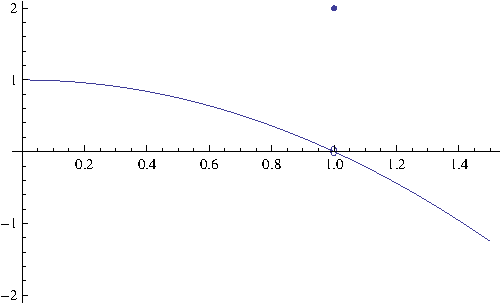
\includegraphics{2_4_8.pdf} \\
	\end{center}
	\end{figure}
\end{solution}
\item
\begin{solution}
	\begin{align*}
		\lim_{x\to 1^+} f(x) &= \boxed{0} \\
		\lim_{x\to 1^-} f(x) &= \boxed{0} 
	\end{align*}
\end{solution}
\item
\begin{solution}
	Yes, the limit does exist and 
	\begin{equation*} \lim_{x\to 1} f(x) = \boxed{0,} \end{equation*}
	since the limit from the left is equal to the limit from the right.
\end{solution}
\ee

\begin{problem}[5.]\S 2.4: 18.
\end{problem}

\be
\item
\begin{solution}
	\begin{align*}
		\lim_{x\to 1^+} \dfrac{\sqrt{2x} (x - 1)}{|x - 1|} 
			&= \lim_{x\to 1^+} \dfrac{\sqrt{2x} (x - 1)}{x - 1} \\
			&= \lim_{x\to 1^+} \sqrt{2x} \\
			&= \boxed{\sqrt{2}.}
	\end{align*}
\end{solution}
\item
\begin{solution}
	\begin{align*}
		\lim_{x\to 1^-} \dfrac{\sqrt{2x} (x - 1)}{|x - 1|} 
			&= -\lim_{x\to 1^+} \dfrac{\sqrt{2x} (x - 1)}{x - 1} \\
			&= -\lim_{x\to 1^+} \sqrt{2x} \\
			&= \boxed{-\sqrt{2}.} 
	\end{align*}
\end{solution}
\ee

\begin{problem}[6.]Compute the following limits:
	\be
		\item $\lim_{t\to0}\Big(\ \dfrac{2t}{\tan(t)}-\dfrac{\sin(\sin(t))}{\sin(t)}\ \Big)$
		\item $\lim_{y\to0}\Big(\ \dfrac{\sin(5y)}{\sin(4y)}+\dfrac{\sin(3y)\cot(5y)}{y\cot(4y)}\ \Big)$\\
	\ee
\end{problem}

\be
\item
\begin{solution}
		\begin{align*}
			\lim_{t\to0}\left(\dfrac{2t}{\tan(t)}-\dfrac{\sin(\sin t)}{\sin t}\right)
				&= \lim_{t\to0}\left(\dfrac{2t \cos t}{\sin t} -
					\dfrac{\sin(\sin t)}{\sin t}\right) \\
			&= 2 \left(\lim_{t\to0} \cos t\right) \cdot \left(\lim_{t\to 0}
				\dfrac{\sin t}{t}\right)^{-1} - \left(\lim_{t\to 0}
				\dfrac{\sin(\sin(t))}{\sin(t)}\right) \\
			&= 2 (\cos 0) \cdot (1)^{-1} - \left(\lim_{t\to 0} \dfrac{\sin(\sin(t))}{\sin(t)}\right) \\
			&= 2 - \left(\lim_{t\to 0} \dfrac{\sin(\sin t)}{\sin t}\right) 
		\end{align*}
		Now we will make the following substitution $u = \sin t$. If $t \to 0$ then
		$\sin t \to 0$ and so $u \to 0$. Putting this together gives
		\begin{equation*}
			\lim_{t\to 0} \dfrac{\sin(\sin t)}{\sin t} = \lim_{u\to 0} \dfrac{\sin
			u}{u}.
		\end{equation*}
		Finally, substitute this into the our original problem and we have
		\begin{align*}
			\lim_{t\to0}\left(\dfrac{2t}{\tan(t)}-\dfrac{\sin(\sin(t))}{\sin(t)}\right)
				&= 2 - \left(\lim_{t\to 0} \dfrac{\sin(\sin(t))}{\sin(t)}\right) \\ 
			&= 2 - \left(\lim_{u\to 0} \dfrac{\sin u}{u}\right) \\
			&= 2 - 1 \\
			&= \boxed{1.}
		\end{align*}
\end{solution}

\item
\begin{solution}
	\begin{align*}
		\lim_{y\to0} \left(\dfrac{\sin(5y)}{\sin(4y)} + \dfrac{\sin(3y)\cot(5y)}{y\cot(4y)}\right)
			&= \left(\lim_{y\to0} \dfrac{\sin(5y)}{\sin(4y)}\right) + \left(\lim_{y\to
		 		0}\dfrac{\sin(3y)\cot(5y)}{y\cot(4y)}\right) \\
		&= \left(\lim_{y\to0} \frac{4}{4} \frac{5}{5} \frac{y}{y}
			\dfrac{\sin(5y)}{\sin(4y)}\right) + \left(\lim_{y\to 0}
			\dfrac{\sin(3y)\cos(5y)\sin(4y)}{y\cos(4y)\sin(5y)}\right) \\
		&= \frac{5}{4}\left(\lim_{y\to0} \frac{4y}{\sin (4y)} \frac{\sin (5y)}{5y}\right) + \left(\lim_{y\to 0}
			\frac{3}{3} \frac{4}{4} \frac{5}{5} \frac{y}{y} \dfrac{\sin(3y)\cos(5y)\sin(4y)}{y\cos(4y)\sin(5y)}\right) \\
		&= \frac{5}{4}\left(\lim_{y\to0} \frac{\sin (4y)}{4y}\right)^{-1}
			\left(\lim_{y\to 0} \frac{\sin (5y)}{5y}\right) \\ & \qquad + \frac{3\cdot 4}{5}
			\left(\lim_{y\to 0} \frac{\cos(5y)}{\cos(4y)}\right)\cdot \left(\lim_{y\to
			0} \dfrac{\sin(3y) \sin(4y) 5y }{3y \cdot 4y \sin(5y)}\right) \\
		&= \frac{5}{4} (1)^{-1} \cdot (1) + \frac{12}{5} \left(
			\frac{\cos(0)}{\cos(0)}\right)\cdot \left(\lim_{y\to 0}\dfrac{\sin(3y)
			\sin(4y) 5y }{3y \cdot 4y \sin(5y)}\right) \\
		&= \frac{5}{4} + \frac{12}{5}\cdot (1)\cdot \left(\lim_{y\to 0}
			\dfrac{\sin(3y)}{3y}\right)\cdot \left(\lim_{y\to 0}
			\dfrac{\sin(4y)}{4y}\right)\cdot \left(\lim_{y \to 0}
			\dfrac{\sin(5y)}{5y}\right)^{-1} \\
		&= \frac{5}{4} + \frac{12}{5}\cdot (1) \cdot (1)\cdot (1)^{-1} \\
		&= \frac{5}{4} + \frac{12}{5} \\
		&= \frac{25 + 48}{20} \\
		&= \boxed{\frac{73}{20}.}
	\end{align*}
\end{solution}
\ee
\end{document}
